\documentclass[9pt,twoside,lineno]{pnas-new}
% Use the lineno option to display guide line numbers if required.

\templatetype{pnassupportinginfo}
\usepackage{longtable}

\title{Reintroduction of resistant frogs allows recovery in the presence of a lethal fungal disease}
\author{Roland A. Knapp, Mark Q. Wilber, Allison Q. Byrne, Maxwell B. Joseph, Thomas C. Smith, Andrew P. Rothstein, Robert L. Grasso, Erica Bree Rosenblum}
\correspondingauthor{Corresponding Author name. Roland A. Knapp \\ E-mail: roland.knapp@ucsb.edu}

\begin{document}

\maketitle

%% Adds the main heading for the SI text. Comment out this line if you do not have any supporting information text.
\SItext
\hypertarget{frog-evolution-in-response-to-bd-2}{%
\section{Frog evolution in response to
Bd}\label{frog-evolution-in-response-to-bd-2}}

\hypertarget{methods}{%
\subsection{Methods}\label{methods}}

We compared frog genomes sampled in naive versus recovering populations.
Bd-exposure histories of these populations are based on a decade or more
of data from visual encounter surveys and Bd surveillance using skin
swabbing \citep[e.g.,][]{knapp2016}. Comparing populations with
different infection histories allowed larger sample sizes and
replication across the landscape. The alternative approach of comparing
samples from the same populations before and after Bd exposure isn't
feasible in this system because Bd arrived in most MYL frog populations
decades ago and population persistence/recovery is rare and
unpredictable. As a result, samples from recovering populations
collected from before and after Bd exposure are not available and are
unlikely to be available in the future.

\hypertarget{results-1}{%
\subsection{Results}\label{results-1}}

In the Results section of the main paper, we describe the stringent set
of outlier SNPS (identified using a Bonferroni-corrected p-value of
0.01). The liberal set, identified using a Bonferroni-corrected p-value
of 0.05, included 38 outliers (35 SNPs and 3 structural variants) from
30 distinct genes across 16 contigs.

Multiple genes in our stringent set of outliers have known associations
with amphibian Bd resistance/tolerance. Of particular interest is a
\textasciitilde940kb region on contig 8 that we identified as under
selection, and that contains 8 genes associated with either the MHC
Class I or Class III regions. The order of these genes in the MYL frog
genome is conserved from \emph{Xenopus} \citep{ohta2006} and is
consistent with MHC Class I/III linkage reported in the Komodo dragon
\citep{reed2021}. Numerous studies have linked MHC genes to frog
resistance/tolerance against Bd infection
\citep[e.g.,][]{savage2011, bataille2015}. In addition to the genes in
this region that we describe in the Results section of the main paper,
other genes also deserve mention. For example, we identified the MHC
Class III gene, heat shock protein 70 (HSP70), as occurring in this
region (Figure~\ref{fig-synteny-plot}). Similarly, \citep{byrne2020}
identified an HSP70-binding protein as a candidate gene under selection
in \emph{Atelopus varius} populations recovering after Bd-caused
declines. HSP70 was also highly expressed in Bd-infected versus
uninfected \emph{Xenopus tropicalis} \citep{rosenblum2009}. This MHC
gene cluster lies on the same chromosome as the outlier SNP in RIN3
(Fig. 2 C), a gene associated with
inflammation response that is highly expressed in amputated
\emph{Xenopus} tails \citep{fukazawa2009}.

Additionally, we identified a region on contig 19 that had the highest
\(\pi_{diff}\) of any outlier window, indicative of directional
selection. This region contained the gene, interferon-induced very large
GTPase 1-like (GVINP1). Interferons boost immune system processes and
previous studies of frogs have identified interferon-related genes as
associated with Bd resistance/tolerance \citep{byrne2020} or have shown
increased expression of this class of genes when frogs were exposed to
Bd in the lab \citep{rosenblum2009, ellison2014}. Variants in GVINP1
also explained approximately 20\% of the resistance to amoebic gill
disease in Atlantic salmon, a finding confirmed via expression analysis
\citep{robledo2018, robledo2020}. Furthermore, in \emph{Litoria
verreauxii alpina}, the related gene, IFN-induced very large GTPase,
showed lower expression in frogs from less susceptible populations
versus more susceptible populations \citep{grogan2018}.

Finally, we identified a region characterized by high
\emph{F\textsubscript{ST}} and low \(\pi_{diff}\) and that contained the
complement genes C6 and C7. This could indicate that balancing selection
is acting in this region of the genome to favor a diverse set of
alleles, as is known for C6 in humans \citep{soejima2005}.

\newpage

\hfill\break

\begin{figure}

{\centering 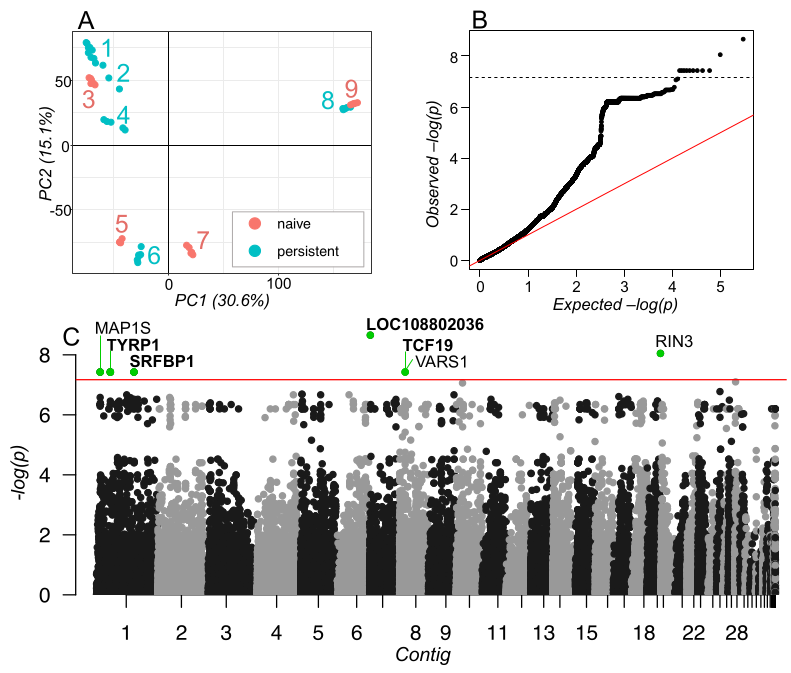
\includegraphics[width=0.8\textwidth]{figures/pca_qq_manhattan.png}

}

\caption{\label{fig-selectionresults}Results from the exome capture
selection study. (A) PCA calculated from binary SNPs showing genomic
relationship of samples. Numeric labels and colors match those in
Fig. 1 A. (B) qqplot showing observed and
expected p-values for 148,307 SNPs and indels as calculated in GEMMA.
Dashed line shows p-value that identifies outliers. (C) Manhattan plot
showing p-values for each SNP as calculated by GEMMA. SNPs are sorted by
genomic position and contigs are sorted by size. Red line shows p-value
that identifies outliers. Outlier SNPs above this threshold are
highlighted and labeled. Bold labels indicate at least one
non-synonymous SNP is present in that gene.\\
}

\end{figure}\clearpage

\begin{figure}

{\centering 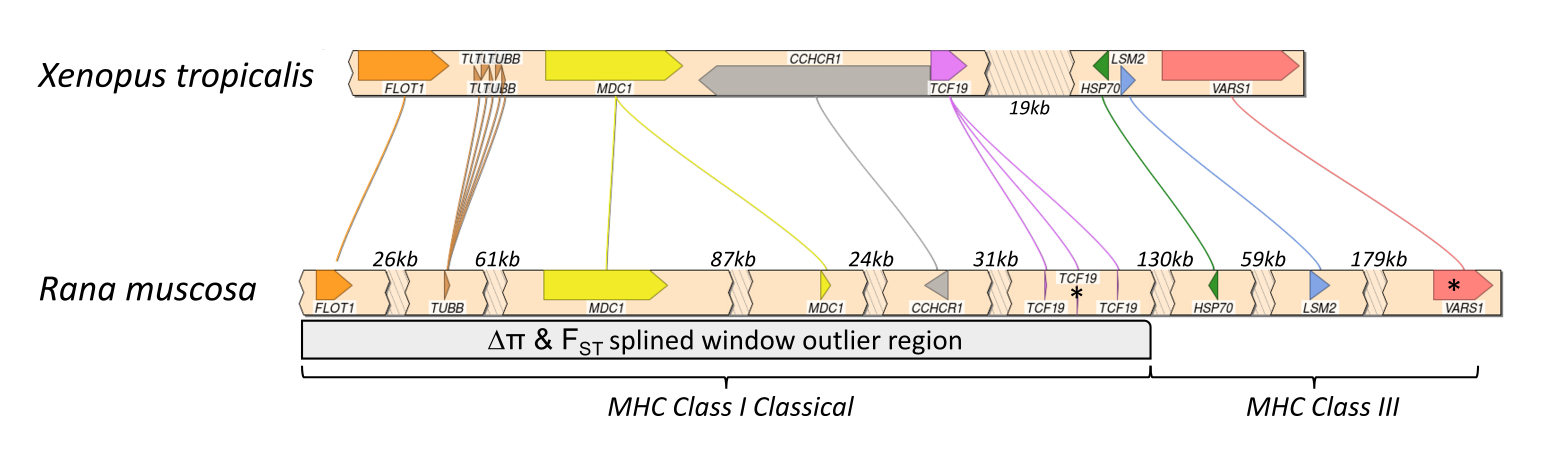
\includegraphics[width=0.8\textwidth]{figures/synteny_figure.png}

}

\caption{\label{fig-synteny-plot}Synteny plot showing conserved gene
order in \emph{Xenopus tropicalis} and \emph{Rana mucosa} for the
outlier region containing MHC Class I Classical and MHC Class III gene
regions. The plot was created with SimpleSynteny \citep{veltri2016}
using \emph{Xenopus tropicalis} Chromosome 8 (NC\_030684.2, genbank
accession GCA\_000004195.4) and \emph{Rana mucosa} Contig19. Asterices
indicate the location of SNP outliers in TCF19 and VARS1 genes. Gap
sizes for each contig representation are labeled.}

\end{figure}\clearpage

\newpage

\begin{figure}

{\centering 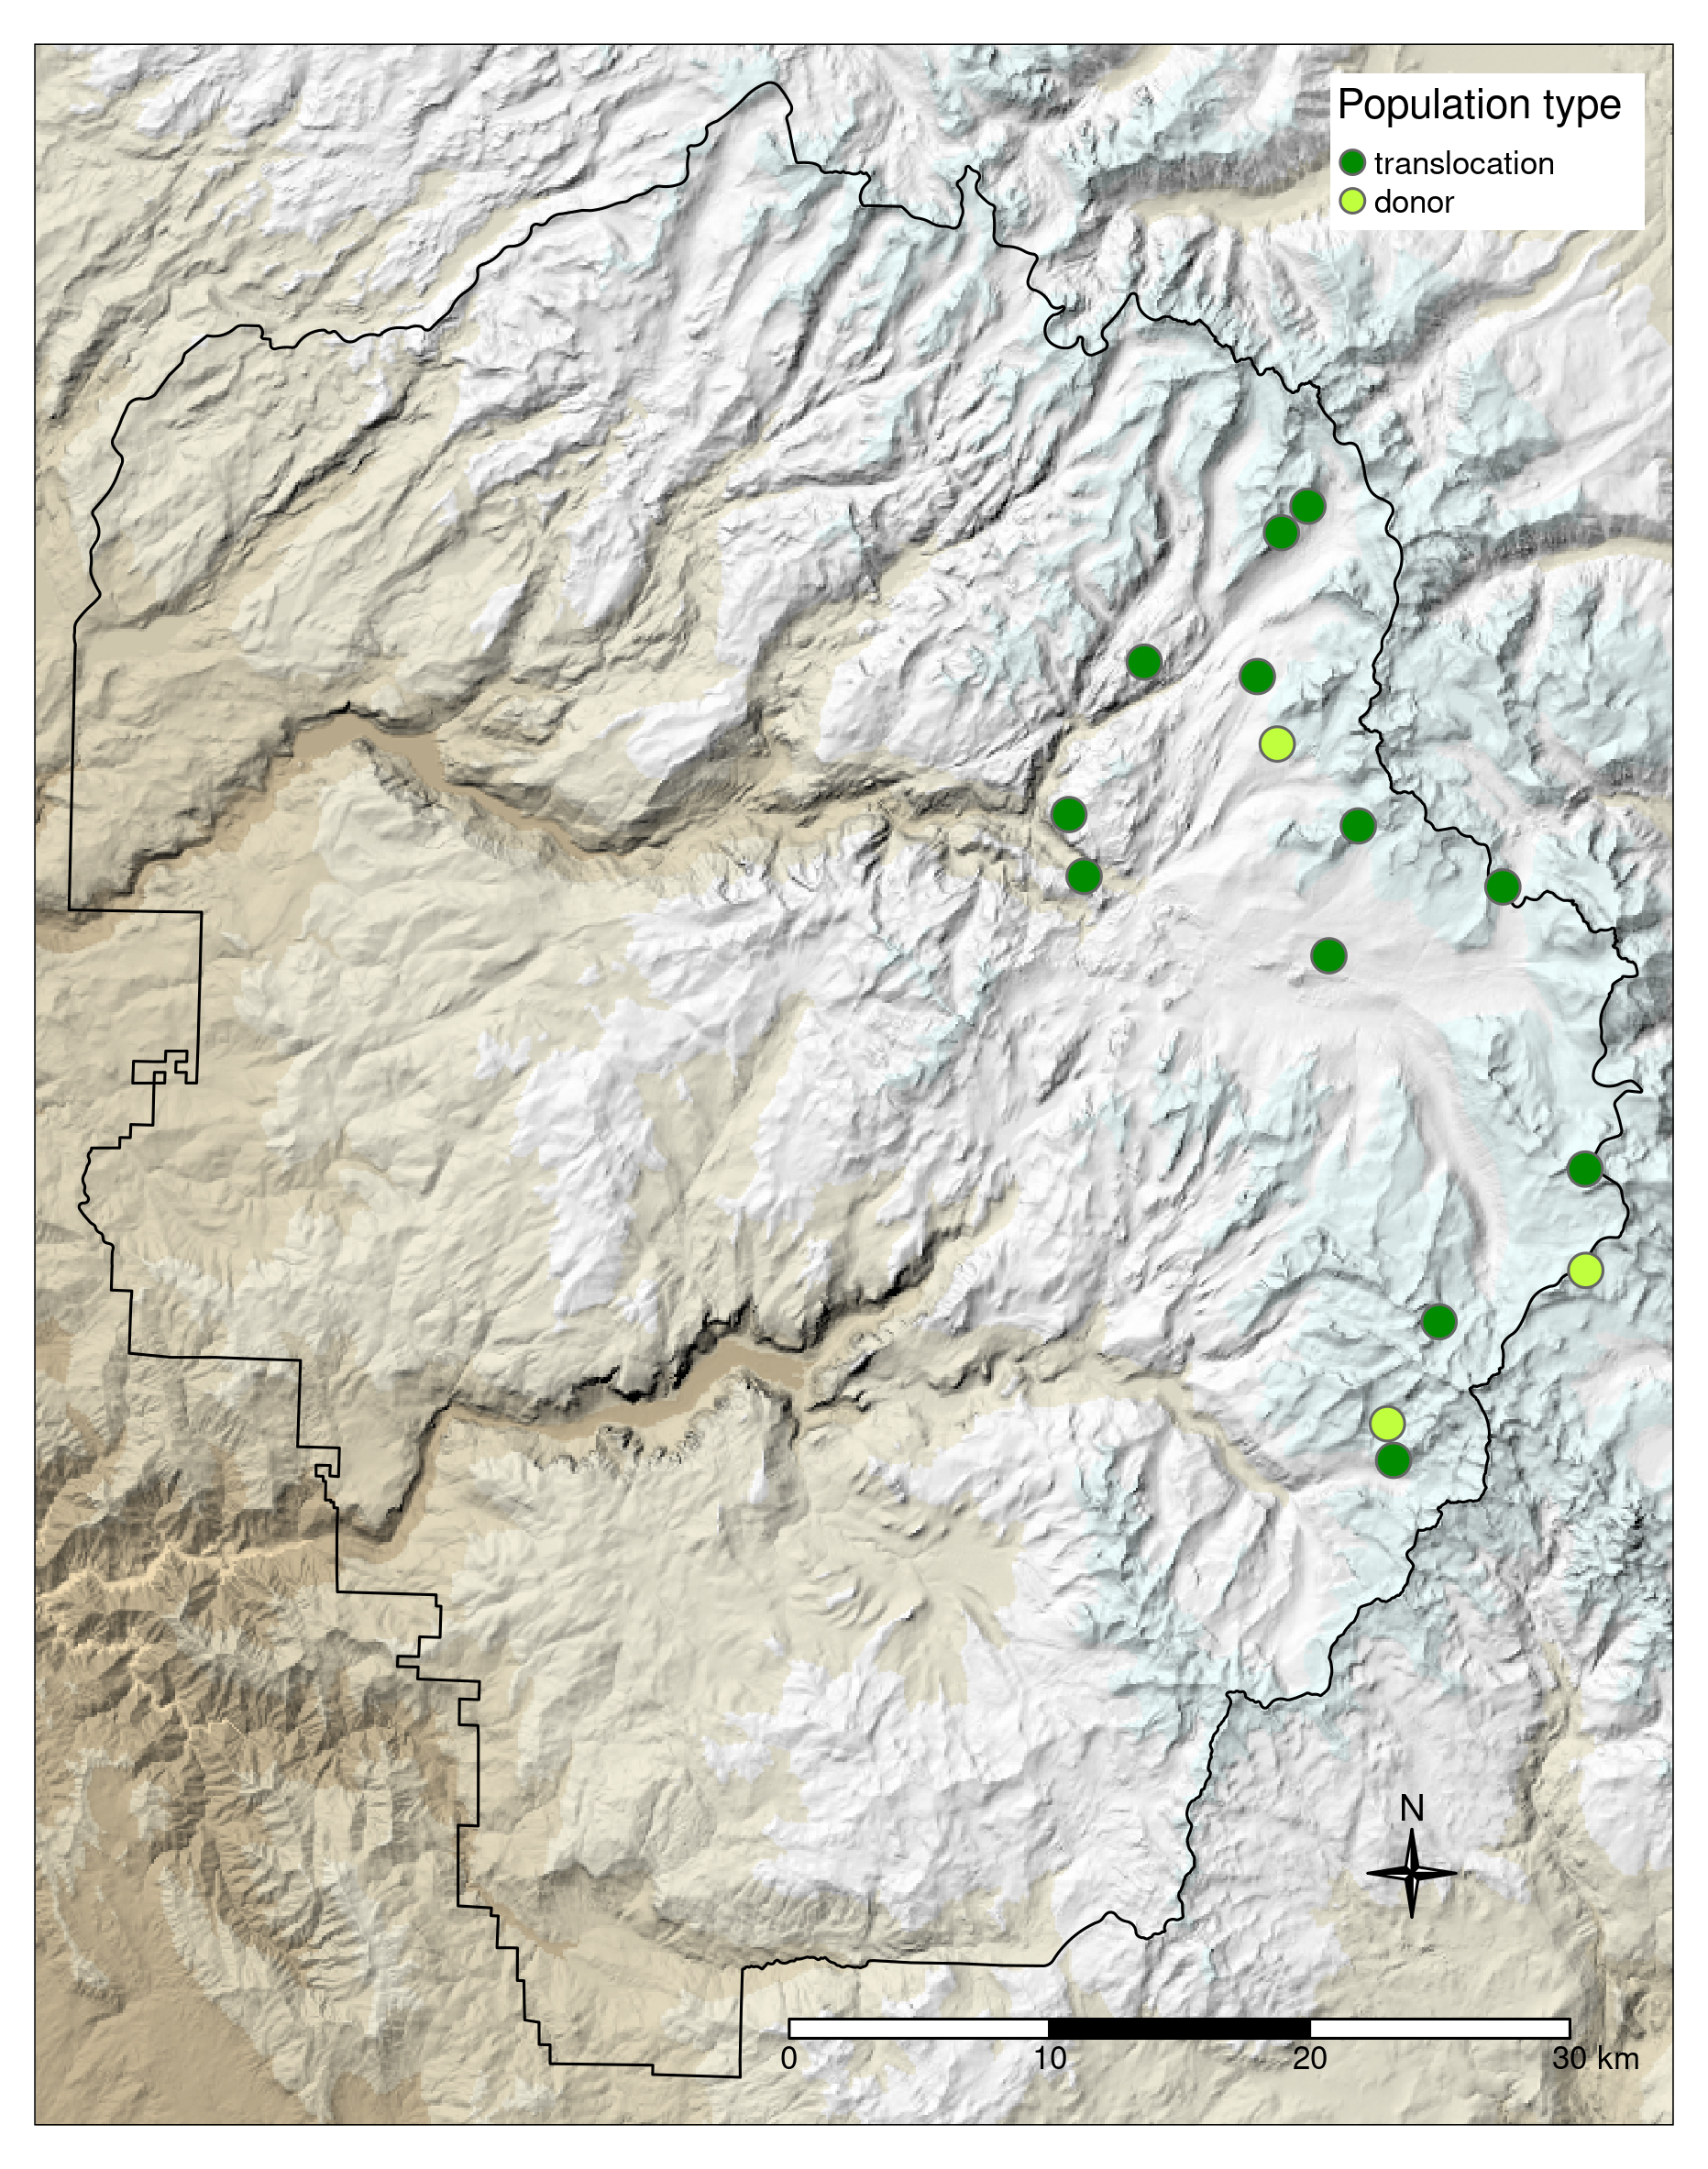
\includegraphics[width=0.8\textwidth]{figures/map_translocation_points.png}

}

\caption{\label{fig-yosemap}Map showing the locations of translocated
and donor MYL frog populations in Yosemite National Park (park boundary
indicated by black polygon). Symbol shapes indicate the donor population
used for each translocation site. To obscure the exact locations of
populations, random noise was added to all point coordinates. Inset map
shows the location of Yosemite within California. In both maps,
elevation is indicated by the colored hillshade layer (dark green =
lowest elevation, white = highest elevation). }

\end{figure}\clearpage

\begin{figure}

{\centering 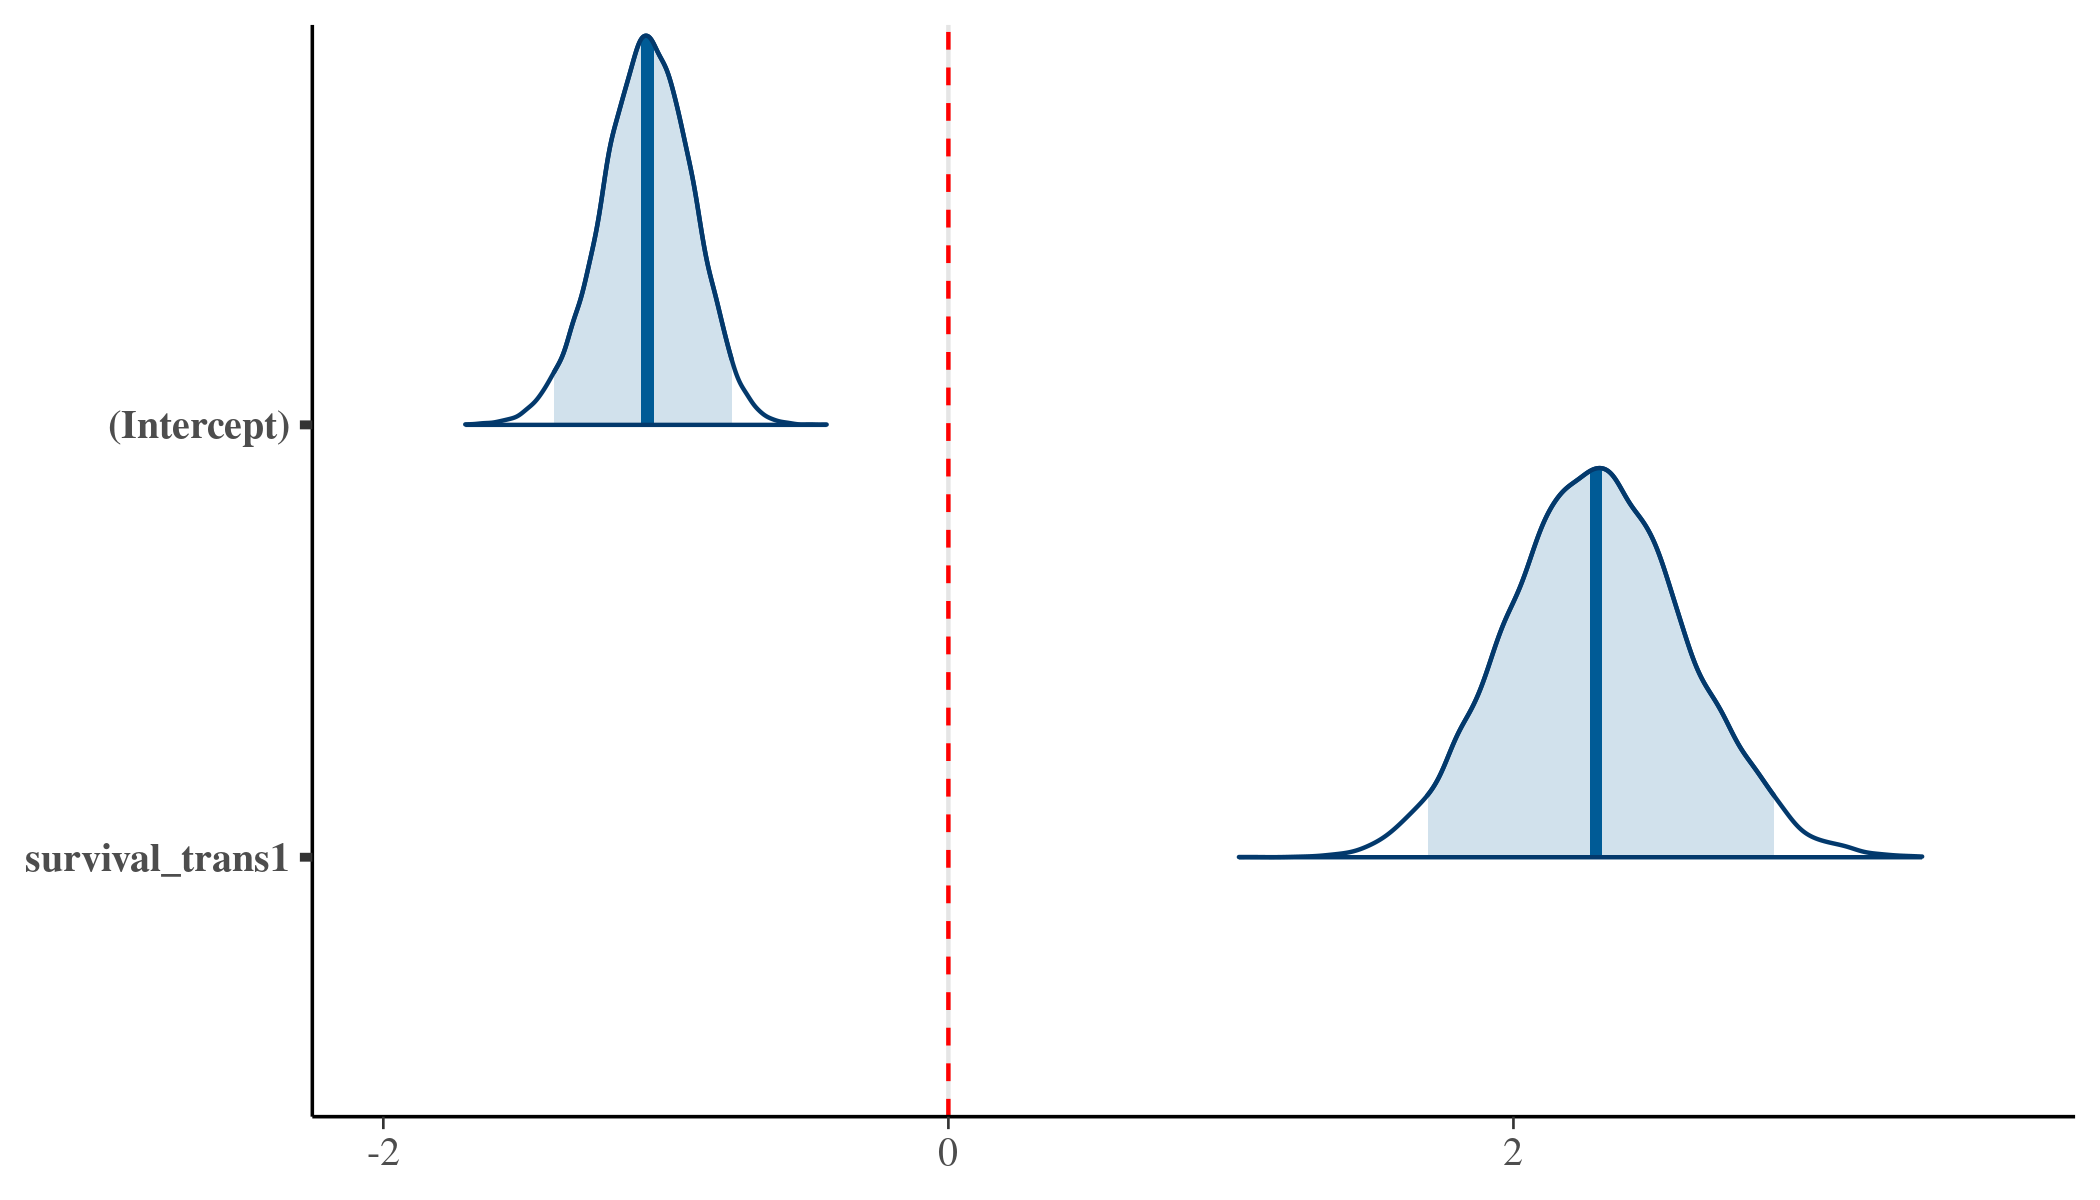
\includegraphics[width=0.8\textwidth]{figures/mcmc_areas_m2b.png}

}

\caption{\label{fig-transsurvival-postdens}For the best model describing
the average 1-year survival of frogs in the first translocation to a
site as a predictor of survival of frogs in all subsequent
translocations to that site, estimated posterior density curves and
shaded 95\% uncertainty intervals for the intercept and single predictor
variable. In the Bayesian framework in which the model was developed, a
variable is considered an important predictor if the associated
uncertainty interval does not overlap zero (indicated by the dashed red
line).}

\end{figure}\clearpage

\begin{figure}

{\centering 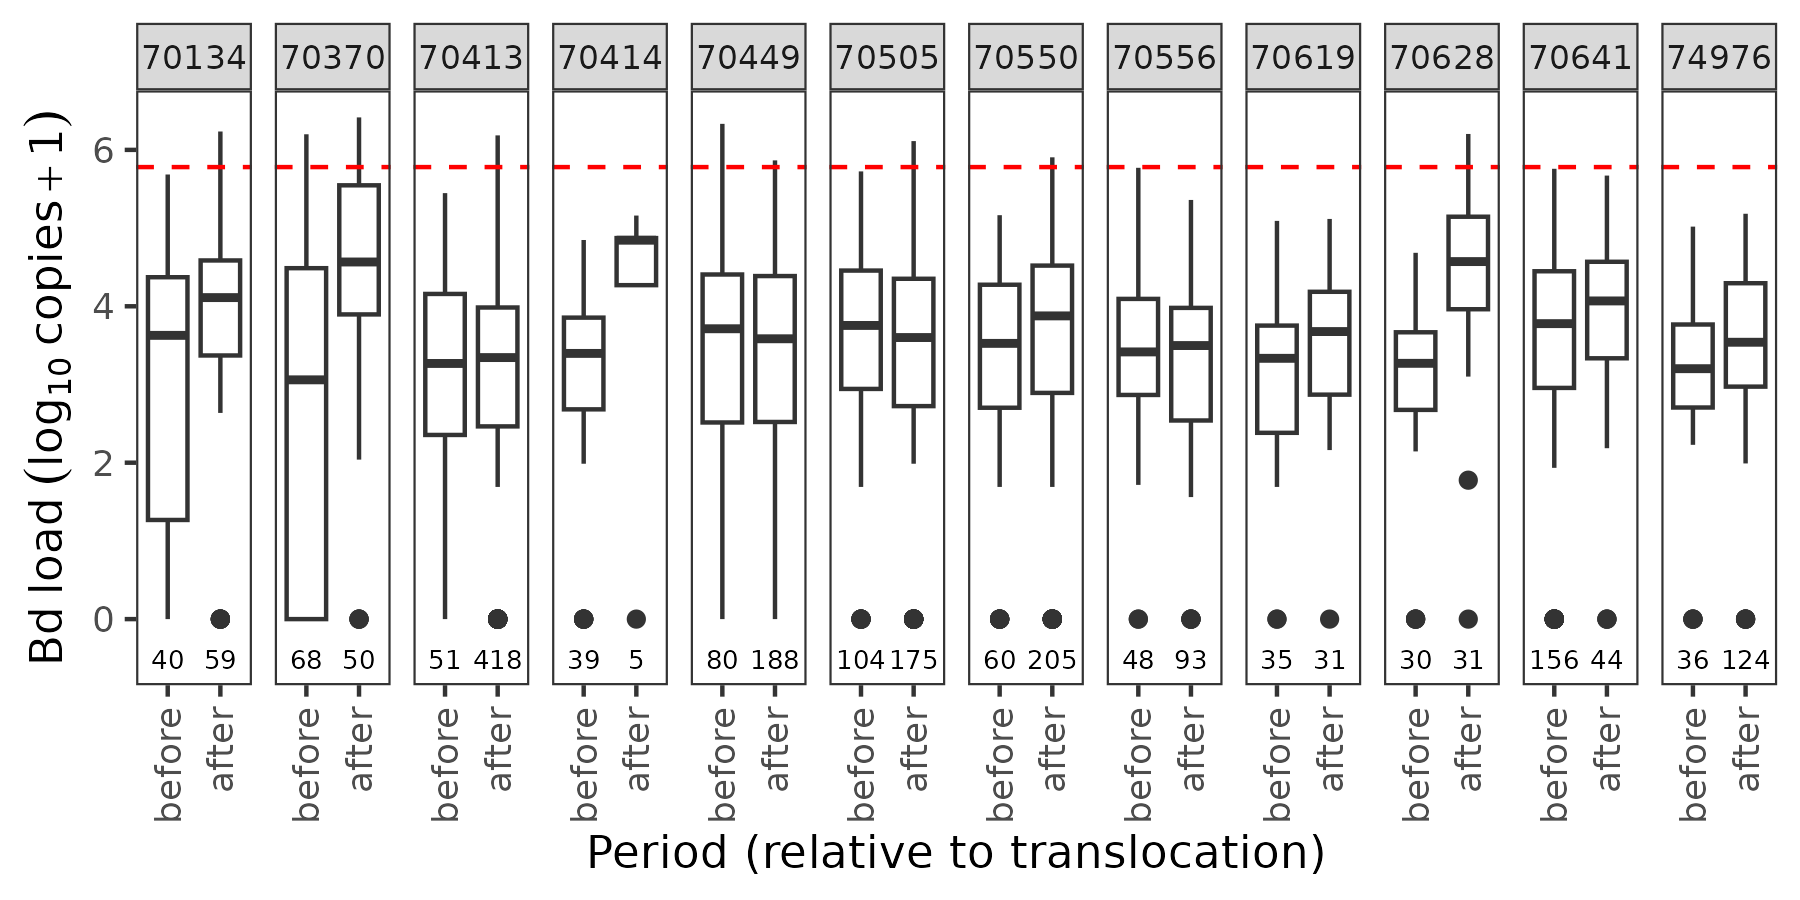
\includegraphics[width=0.8\textwidth]{figures/bdload_beforeafter.png}

}

\caption{\label{fig-bdload-beforeafter}For frogs translocated to each of
the 12 recipient sites, Bd loads for the period immediately prior to
translocation versus during the 1-year period after translocation. Box
plot details are as in Fig. 4.}

\end{figure}\clearpage

\begin{figure}

{\centering 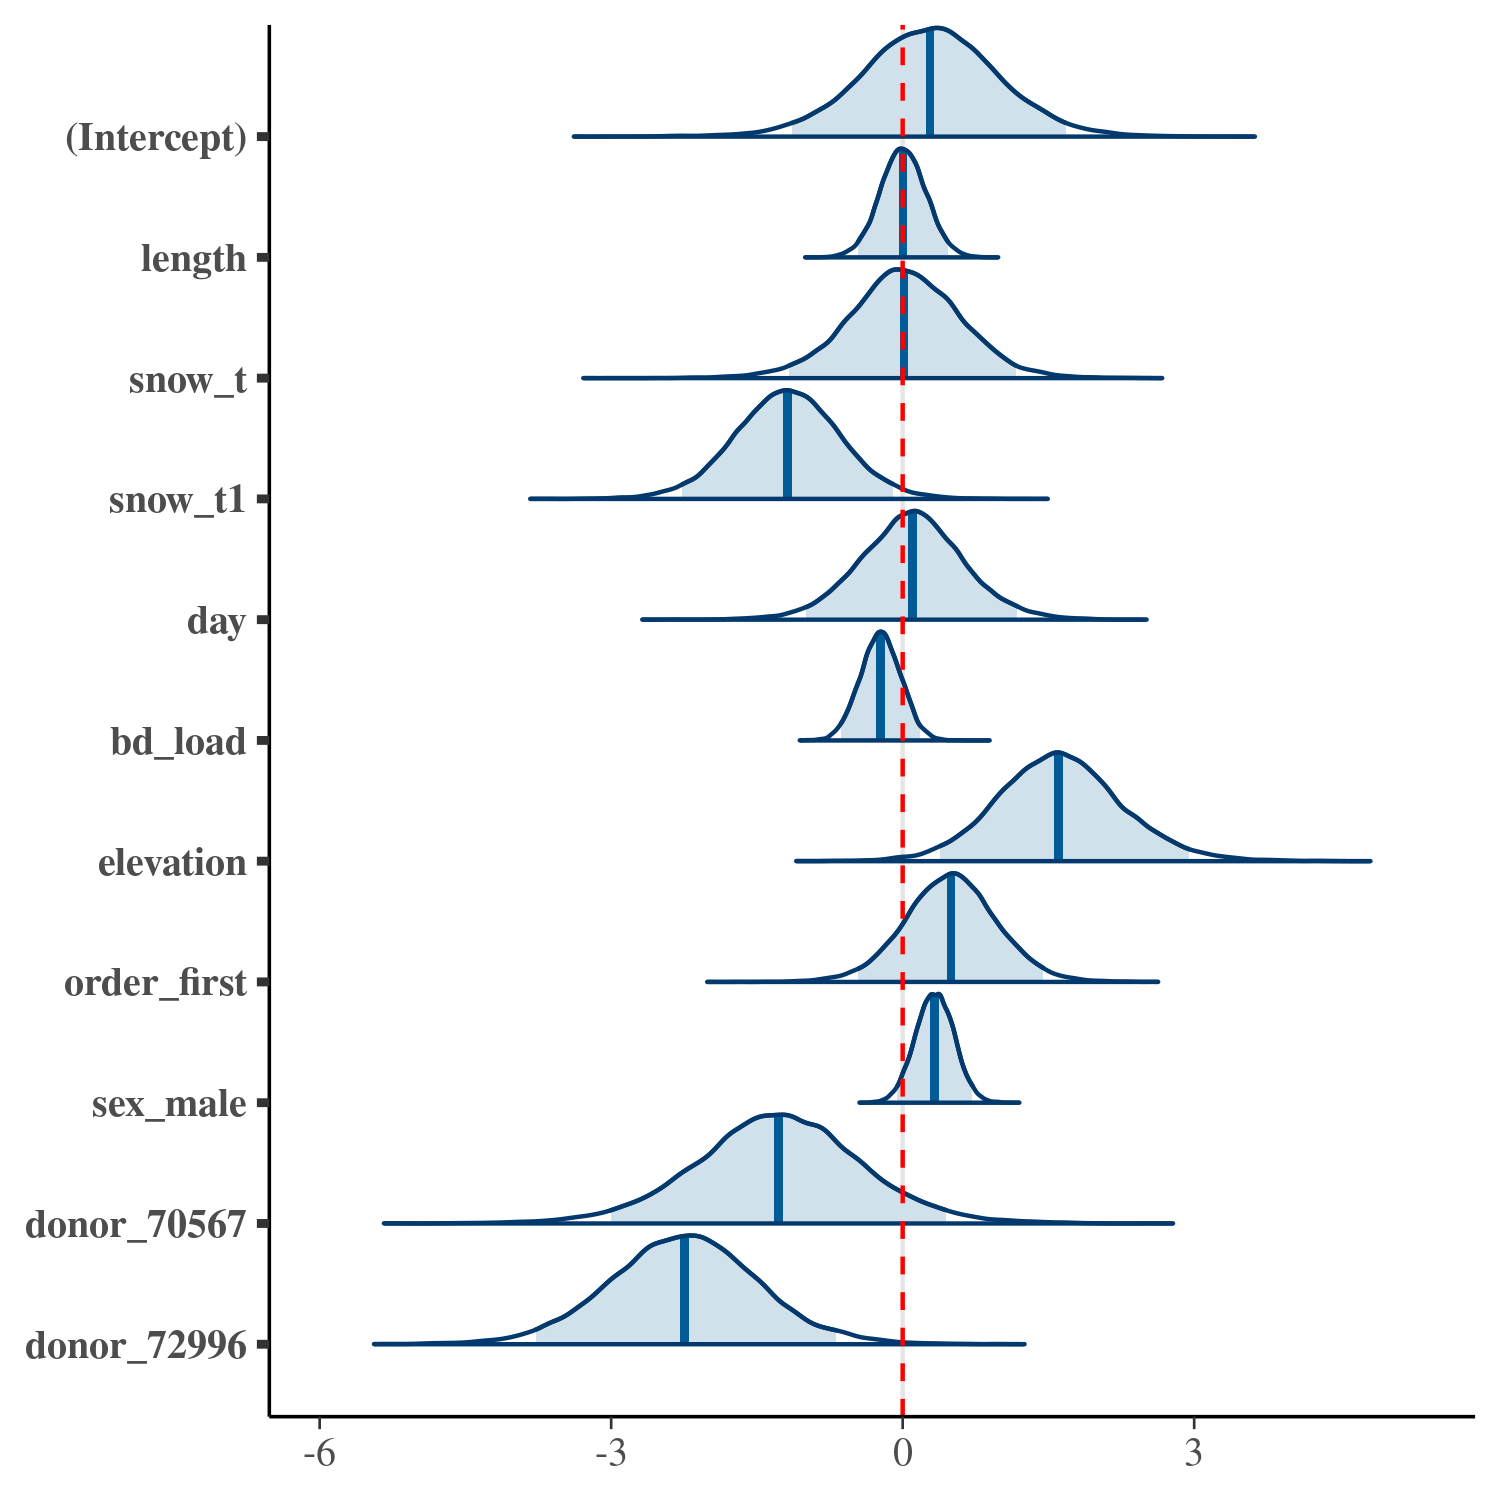
\includegraphics[width=0.8\textwidth]{figures/mcmc_areas_m1d.png}

}

\caption{\label{fig-survival-postdens}For the best model identifying
predictors of 1-year frog survival following translocation, estimated
posterior density curves and shaded 95\% uncertainty intervals for the
intercept and all predictor variables. In the Bayesian framework in
which the model was developed, variables are considered important
predictors if the associated uncertainty interval does not overlap zero
(indicated by the dashed red line).}

\end{figure}\clearpage

\begin{figure}

{\centering 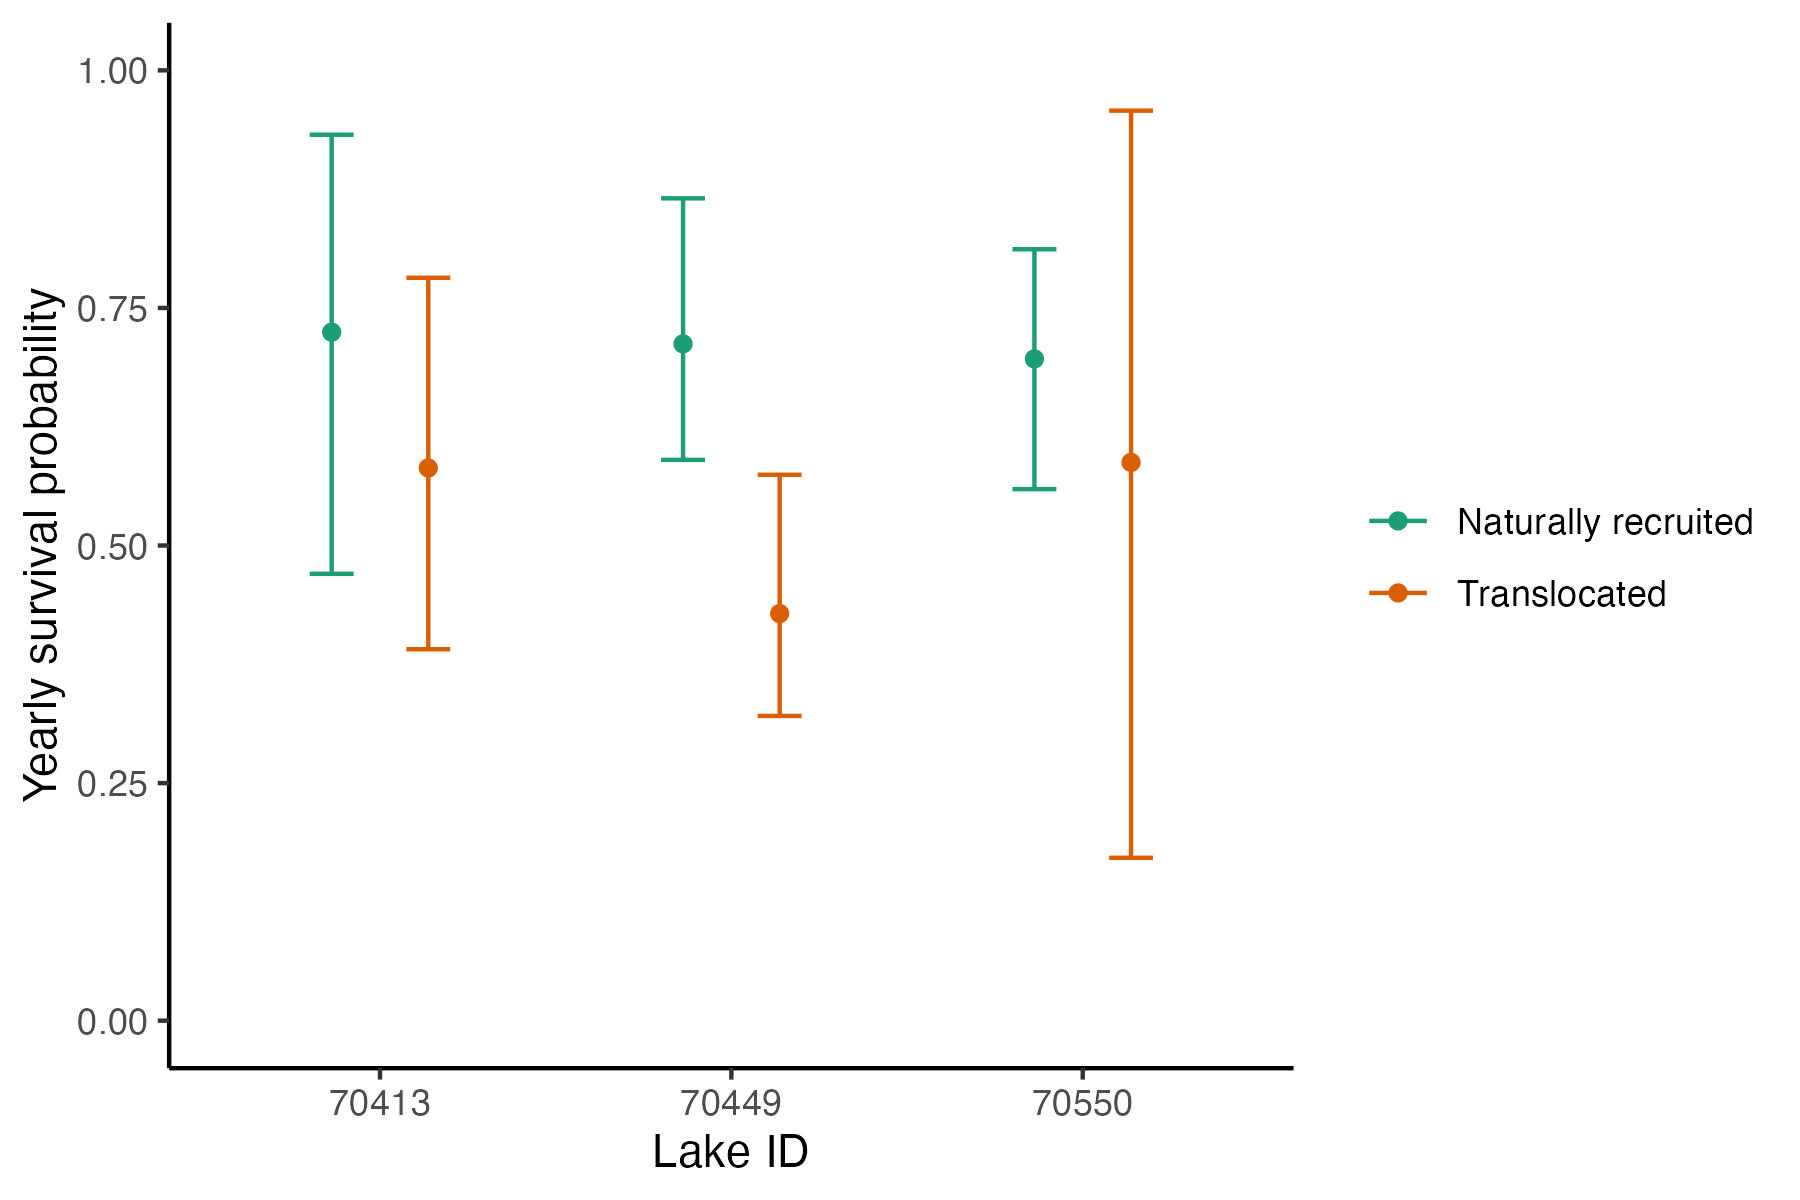
\includegraphics[width=0.8\textwidth]{figures/compare_surv_probs.jpg}

}

\caption{\label{fig-compare_surv_probs}Comparison of the average yearly
adult survival probabilities for adults translocated to each of three
sites versus adults that were naturally recruited at each site (as a
result of reproduction by translocated frogs). In contrast to
Fig. 3, these are not survival
probabilities from the first year following translocation, but instead
represent averaged survival probabilities across multiple years and
cohort. Points are median estimates and error bars give the 95\%
uncertainty intervals around the estimates, accounting for yearly
variation in survival probabilities. The large error bars for 70550
reflect the large within and among individual variability in yearly
survival probability at this site (as also reflected in one-year
survival probabilities in Fig. 3). All
estimates are derived from the mrmr package.}

\end{figure}\clearpage

\newpage

\hypertarget{tables}{%
\subsubsection{Tables}\label{tables}}

\hfill\break



\hypertarget{tbl-survival-earlylate}{}
\begin{longtable}[]{@{}
  >{\raggedright\arraybackslash}p{(\columnwidth - 8\tabcolsep) * \real{0.0654}}
  >{\centering\arraybackslash}p{(\columnwidth - 8\tabcolsep) * \real{0.2056}}
  >{\centering\arraybackslash}p{(\columnwidth - 8\tabcolsep) * \real{0.2430}}
  >{\centering\arraybackslash}p{(\columnwidth - 8\tabcolsep) * \real{0.2056}}
  >{\centering\arraybackslash}p{(\columnwidth - 8\tabcolsep) * \real{0.2804}}@{}}
\caption{\label{tbl-survival-earlylate}Association between the
proportion of populations translocated early versus late in the study
period (\textless{} 2013 or \textgreater= 2013, respectively) and
probability of survival (\textless{} 0.5 or \textgreater= 0.5). Based on
the viability analysis, survival probabilities \textless{} 0.5 and
\textgreater= 0.5 produced 50-year extinction probabilities of 1 and
\textless{} 0.5, respectively.}\tabularnewline
\toprule()
\begin{minipage}[b]{\linewidth}\raggedright
Period
\end{minipage} & \begin{minipage}[b]{\linewidth}\centering
Survival probability
\end{minipage} & \begin{minipage}[b]{\linewidth}\centering
Number of translocations
\end{minipage} & \begin{minipage}[b]{\linewidth}\centering
Total translocations
\end{minipage} & \begin{minipage}[b]{\linewidth}\centering
Proportion of translocations
\end{minipage} \\
\midrule()
\endfirsthead
\toprule()
\begin{minipage}[b]{\linewidth}\raggedright
Period
\end{minipage} & \begin{minipage}[b]{\linewidth}\centering
Survival probability
\end{minipage} & \begin{minipage}[b]{\linewidth}\centering
Number of translocations
\end{minipage} & \begin{minipage}[b]{\linewidth}\centering
Total translocations
\end{minipage} & \begin{minipage}[b]{\linewidth}\centering
Proportion of translocations
\end{minipage} \\
\midrule()
\endhead
early & \textless{} 0.5 & 4 & 5 & 0.800 \\
early & \textgreater= 0.5 & 1 & 5 & 0.200 \\
late & \textless{} 0.5 & 2 & 7 & 0.286 \\
late & \textgreater= 0.5 & 5 & 7 & 0.714 \\
\bottomrule()
\end{longtable}

\newpage

\hypertarget{tbl-param_values}{}
\begin{longtable}[]{@{}
  >{\raggedright\arraybackslash}p{(\columnwidth - 4\tabcolsep) * \real{0.4545}}
  >{\raggedright\arraybackslash}p{(\columnwidth - 4\tabcolsep) * \real{0.1333}}
  >{\raggedright\arraybackslash}p{(\columnwidth - 4\tabcolsep) * \real{0.4121}}@{}}
\caption{\label{tbl-param_values}Description and values of parameters
used in the model. All survival probabilities are in the presence of the
fungal pathogen Bd.}\tabularnewline
\toprule()
\begin{minipage}[b]{\linewidth}\raggedright
\textbf{Parameter}
\end{minipage} & \begin{minipage}[b]{\linewidth}\raggedright
\textbf{Value}
\end{minipage} & \begin{minipage}[b]{\linewidth}\raggedright
\textbf{Source}
\end{minipage} \\
\midrule()
\endfirsthead
\toprule()
\begin{minipage}[b]{\linewidth}\raggedright
\textbf{Parameter}
\end{minipage} & \begin{minipage}[b]{\linewidth}\raggedright
\textbf{Value}
\end{minipage} & \begin{minipage}[b]{\linewidth}\raggedright
\textbf{Source}
\end{minipage} \\
\midrule()
\endhead
\(\sigma_{L_1}\), Yearly survival probability of year 1 tadpoles & 0.7 &
Estimated from field data, observations, natural history knowledge \\
\(\sigma_{L_2}\), Yearly survival probability of year 2 tadpoles & 0.7 &
Estimated from field data, observations, natural history knowledge \\
\(\sigma_{L_3}\), Yearly survival probability of year 3 tadpoles & 0.7 &
Estimated from field data, observations, natural history knowledge \\
\(\sigma_{J_1}\), Yearly survival probability of year 1 juveniles & 0.25
& Estimated from field data, observations, natural history knowledge \\
\(\sigma_{J_2}\), Yearly survival probability of year 2 juveniles & 0.5
& Estimated from field data, observations, natural history knowledge \\
\(\sigma_{A_R}\), Yearly survival probability of naturally recruited
adults & Varies by population & Estimated from mark-recapture studies \\
\(\sigma_{A_T}\), Yearly survival probability of translocated adults &
Varies by population & Estimated from mark-recapture studies \\
\(p_{L_1}\), Probability of a year 1 tadpoles remaining as a tadpoles &
1 & Estimated from field data, observations, natural history
knowledge \\
\(p_{L_2}\), Probability of a year 2 tadpoles remaining as a tadpoles &
0.25 & Estimated from field data, observations, natural history
knowledge \\
\(p_{J_1}\), Probability of a year 1 juvenile remaining as a juvenile &
0.25 & Estimated from field data, observations, natural history
knowledge \\
\(p_F\), Probability of a adult female reproducing in a year & 0.5 &
Could be as high at 1, based on field observations \\
\(F\), Number of surviving eggs produced by an adult female & 100 & From
observations of captive frogs \\
\(\omega\), Probability of juvenile successfully recruiting to an adult
& Varies yearly & Explored different values of this parameter \\
\bottomrule()
\end{longtable}

\hfill\break


%%% Add this line AFTER all your figures and tables
\FloatBarrier

\dataset{gemma\_outliers.csv}{Description needed}

\dataset{spline\_window\_shared\_outliers.csv}{Description needed}

\bibliography{translocation}

\end{document}

